\documentclass{article}
\usepackage{mystyle}

\title{Notes on binned spherical harmonic expansion implementation}
\author{Scott Trinkle}
\date{Last edited: \today}
\begin{document}
\maketitle

\section{Introduction}
The two major steps in the pipeline for constructing a fiber orientation
distribution (FOD) from a cubic ROI of x-ray \uct data are (1) estimate the
local orientation at each voxel using structure tensor analysis, and (2) express
the distribution of these orientations using the spherical harmonics. Until now,
calculating the relevant spherical harmonic coefficients has been the major
computation bottleneck in this pipeline. This report details a new method for
calculating these coefficients using a spherical binning algorithm that improves
performance by nearly 100\% with no significant drop in accuracy.

\section{Previous implementation}
\subsection{From orientations to FOD}
The output of the structure tensor analysis algorithm for an ROI with a total of
$K$ elements is an array of $K$ vectors: \{$x_k, y_k, z_k$\}. With the current
implementation, these $K$ vectors are first converted into spherical
coordinates: \{$\theta_k, \phi_k$\} with $\theta \in [0, \pi]$ and
$\phi \in [0, 2\pi]$. The FOD is then represented as a sum of dirac delta
functions at these coordinates:
\begin{align}
  \label{eq:1}
  \text{FOD}(\theta, \phi) = \frac{1}{K}\sum_{k=1}^K \delta(\theta - \theta_k)\delta(\phi - \phi_k).
\end{align}

\subsection{Spherical harmonic representation}
The spherical harmonics are defined as
\begin{align}
  Y_l^m(\theta, \phi) = N_l^m P_l^m(\text{cos}\theta)e^{jm\phi},
\end{align}
where $N_l^m$ is a normalization coefficient, and $P_l^m$ are the
associated Legendre polynomials.

The SH form an orthonormal basis over $L_2(\mathbb{S}^2)$. Any
square integrable function $g(\theta, \phi) \in L_2(\mathbb{S}^2)$ can
be expressed as a linear combination of SH:
\begin{align}
  g(\theta, \phi) = \sum_{l=0}^{\infty}\sum_{m=-l}^l c_{lm}Y_l^m(\theta, \phi),
  \label{eq:SHexpand}
\end{align}
with coefficients $c_{lm}$ given by
\begin{align}
  c_{lm} = \int_{\mathbb{S}^2} g(\theta, \phi) \bar{Y}_l^m(\theta, \phi) \mathrm{d}\bm{\Omega},
  \label{eq:coeffs_0}
\end{align}
where the overbar denotes conjugation.

If we substitute Eqn. \ref{eq:1} into Eqn \ref{eq:coeffs_0}, then the sifting property of the Dirac
delta function can be used, and the integral reduces to:
\begin{align}
  c_{lm} = \frac{1}{K}\sum_{k=1}^K \bar{Y}_l^m(\theta_k, \phi_k).
  \label{eq:get_coeffs}
\end{align}
A SH approximation $\hat{\text{FOD}}(\theta, \phi)$ can then be determined to an arbitrary
band-limit $L_{max}$ using Eqn \ref{eq:SHexpand}.

Spherical harmonics are used extensively in the HARDI literature to represent
FODs. Generally, it is assumed that diffusion has antipodal
symmetry, so odd-ordered SH components are assumed to be zero and
ignored. Furthermore, since the diffusion-weighted signal and ODF are both real
functions, their SH representations exhibit conjugate symmetry:
\begin{align}
  Y_{l}^m(\theta, \phi)_{real} \equiv
  \begin{cases}
    \sqrt{2}\text{Re}\left[Y_l^{|m|}(\theta, \phi)\right] & m < 0\\
    Y_l^0(\theta, \phi) & m = 0\\
    \sqrt{2}\text{Im}\left[Y_l^m(\theta, \phi)\right] & m > 0\\
  \end{cases}
  \label{eq:real_Y}
\end{align}

These simplifications hold true for the \uct FODs as well. In this work, we use a
band-limit of $L_{max} = 20$, for a total number of 231 even-ordered SH coefficients.

\subsection{Computational Expense}
With our current data, the \uct voxels are 1.2 $\upmu$m$^3$ isotropic, and the
MRI voxels are 150 $\upmu$m$^3$ isotropic. Accordingly, one MRI-voxel-sized ROI
includes a total of $K=125^3\approx 2$ million \uct voxels. The above
implementation thus requires each of the 231 even spherical harmonics up to
$L_{max}=20$ to be evaluated at 2 million points. Calculating all 231 of these
coefficients with this method for one ROI typically takes around 100 seconds on
the bigmem SIRAF nodes. There are approximately 500,000 voxels in the MRI data.
In order to create a corresponding \uct FOD for each of these voxels with this
method would thus take: 500,000 voxels $\times$ 100 seconds/voxel $\approx$
14,000 hours of computation time, not including the additional time needed
to estimate the orientations themselves.

\section{New implementation: spherical binning}
\subsection{From orientations to FOD}
Representing the FOD as a sum of $K\approx 2 \times 10^6$ delta functions
required each of the spherical harmonics to be evaluated at $K$ points. With the
new method, the FOD is instead constructed as a histogram on the sphere using
$N \ll K$ approximately uniform sampling points as the bin centers. The $N$
sampling points are chosen using a Fibonacci sampling
algorithm~\cite{Hannay2004}. The $K$ vectors are sorted into the corresponding
bins using a very fast nearest-neighbors search algorithm, implemented with a
\href{https://en.wikipedia.org/wiki/Ball_tree}{``ball tree''} nested data
structure in the
\href{http://scikit-learn.org/stable/modules/generated/sklearn.neighbors.NearestNeighbors.html#sklearn.neighbors.NearestNeighbors}{\texttt{scikit-learn}}
Python package.

This ``binned'' FOD can be written as a weighted sum of $N$ delta functions:
\begin{align}
  \label{eq:3}
  \text{FOD}_b = \frac{1}{K}\sum_{n=1}^N b_n \delta(\theta - \theta_n)\delta(\phi - \phi_n),
\end{align}
where $b_n$ is the bin count for the sampling point ($\theta_n, \phi_n$), and
$\sum_n b_n = K$.

\subsection{Spherical harmonic representation}
The calculation of the spherical harmonic coefficients proceeds in the same way. The
``binned'' FOD is substituted into Eqn \ref{eq:coeffs_0}, which results in:
\begin{align}
  c_{lm} = \frac{1}{K}\sum_{n=1}^N b_n \bar{Y}_l^m(\theta_n, \phi_n).
  \label{eq:4}
\end{align}
The same symmetries are exploited from Eqn \ref{eq:real_Y}.

\section{Results}
\subsection{Raw FOD visualization}
An MRI-voxel-sized ROI (125$\times$125$\times$125 voxels) was taken from \uct
data, and the orientations at each voxel were estimated with structure tensor
analysis. For the purposes of this report, orientations were not thresholded by
FA or pixel value to mask out non-fiber voxels.

One advantage to the new binning method is that it allow us to directly
visualize the raw FOD before expanding it onto spherical harmonics. Figure
\ref{fig:fod_raw} is a plot of this FOD calculated according to Eqn~\ref{eq:3}
with $N=6500$. Notably, the raw FOD does not have antipodal symmetry. This is
not surprising --- the orientations at each voxel are calculated as eigenvectors
of a tensor. These normalized eigenvectors are unique within a minus sign; at
each voxel, the opposite orientation might as well have been
reported. Furthermore, the FODs calculated with the dMRI methods of interest
will always have antipodal symmetry. Accordingly, the true \uct FOD we are
interested in estimating is shown in Figure~\ref{fig:fod_even}, which was
calculated by taking every point from Figure~\ref{fig:fod_raw} and assigning the
same bin count to the opposite point. Note that we are already enforcing this
symmetry in the SH representation by only using even-ordered coefficients. I
tested calculating the coefficients from the FODs in both Fig~\ref{fig:fod_raw}
and Fig~\ref{fig:fod_even} and they were identical.



\begin{figure}[h]
  \centering
  \begin{subfigure}[b]{0.48\textwidth}
    \centering
    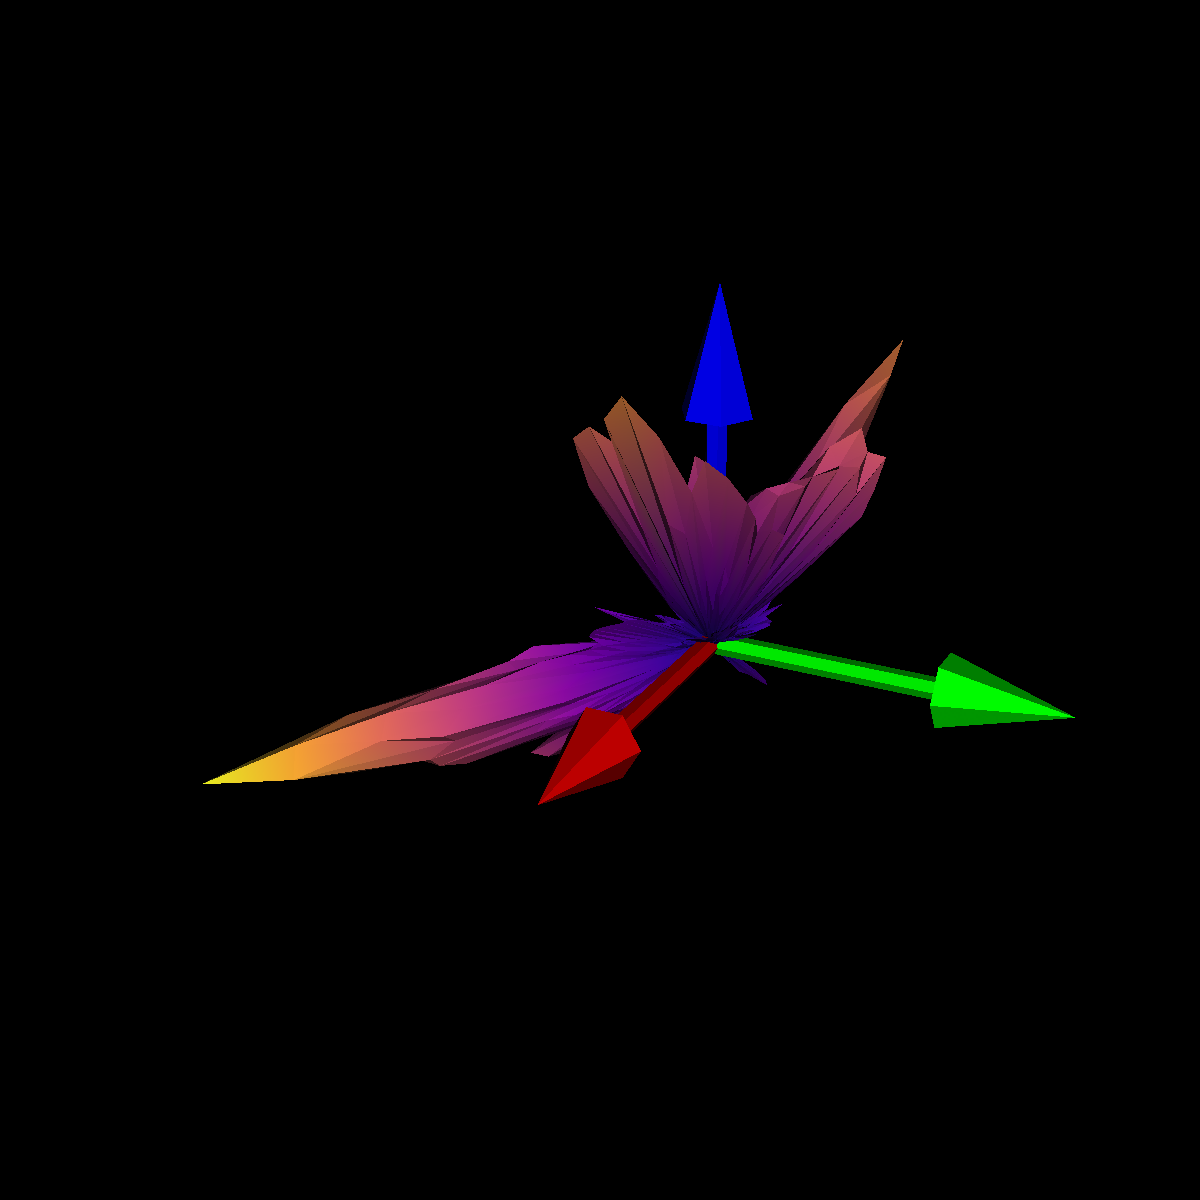
\includegraphics[width=0.9\linewidth]{../odf_comparison/raw_odf}
    \caption{Raw orientations}
    \label{fig:fod_raw}
  \end{subfigure}
  \hspace{0.5em}
  \begin{subfigure}[b]{0.48\textwidth}
    \centering
    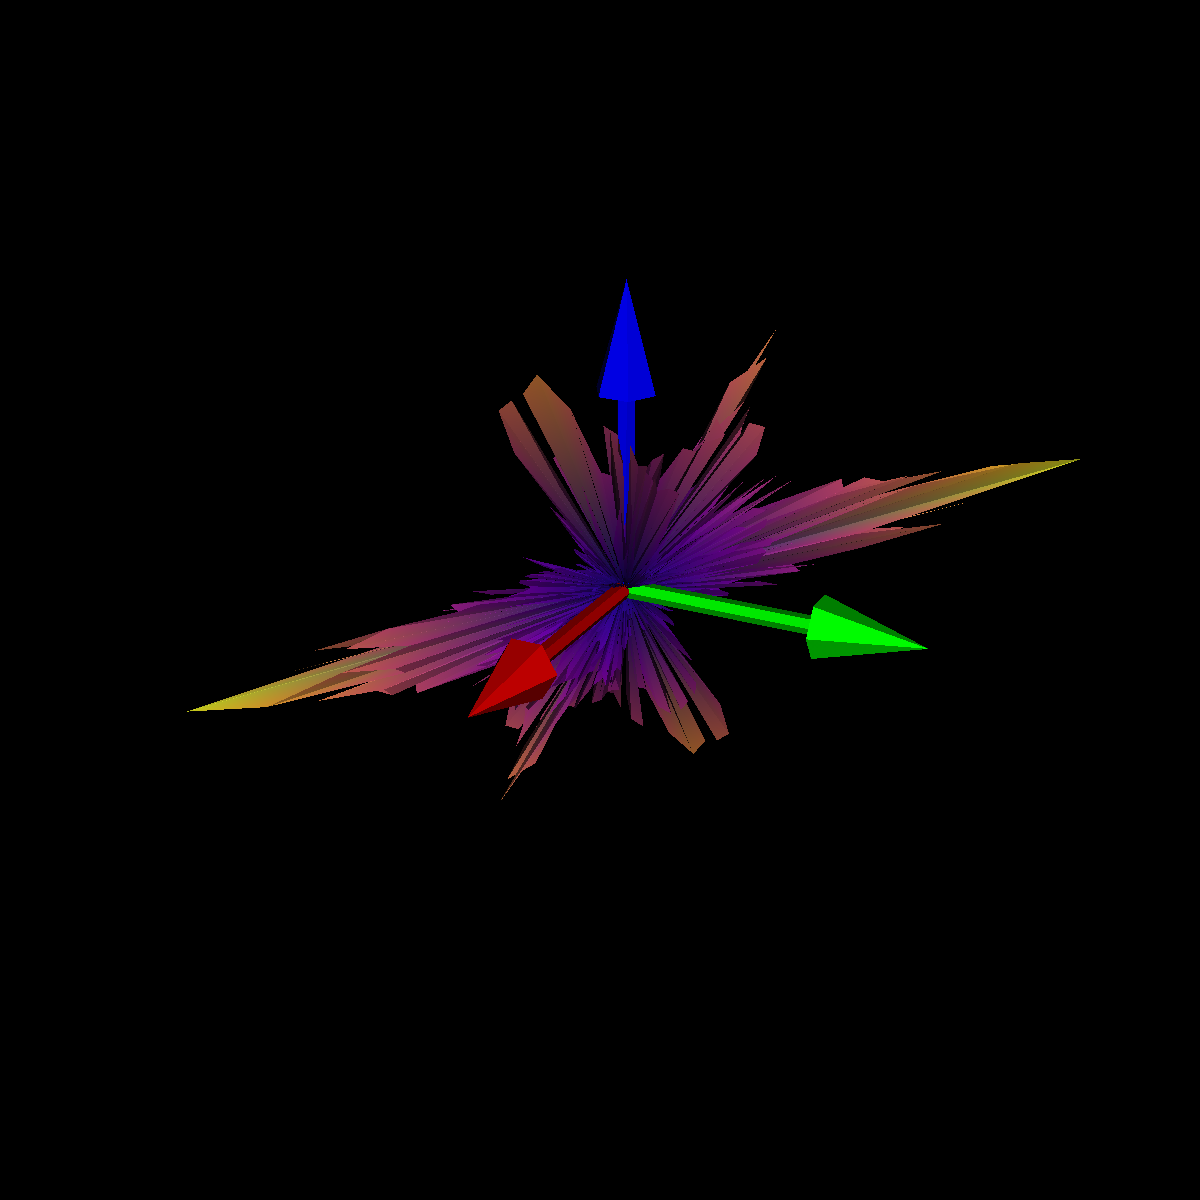
\includegraphics[width=0.9\linewidth]{../odf_comparison/raw_odf_even}
    \caption{After enforcing antipodal symmetry}
    \label{fig:fod_even}
  \end{subfigure}
  \caption{The ``binned'' \uct FOD}
\end{figure}

\subsection{Comparison of methods}
\begin{figure}[h]
  \centering
  \begin{subfigure}[b]{0.48\textwidth}
    \centering
    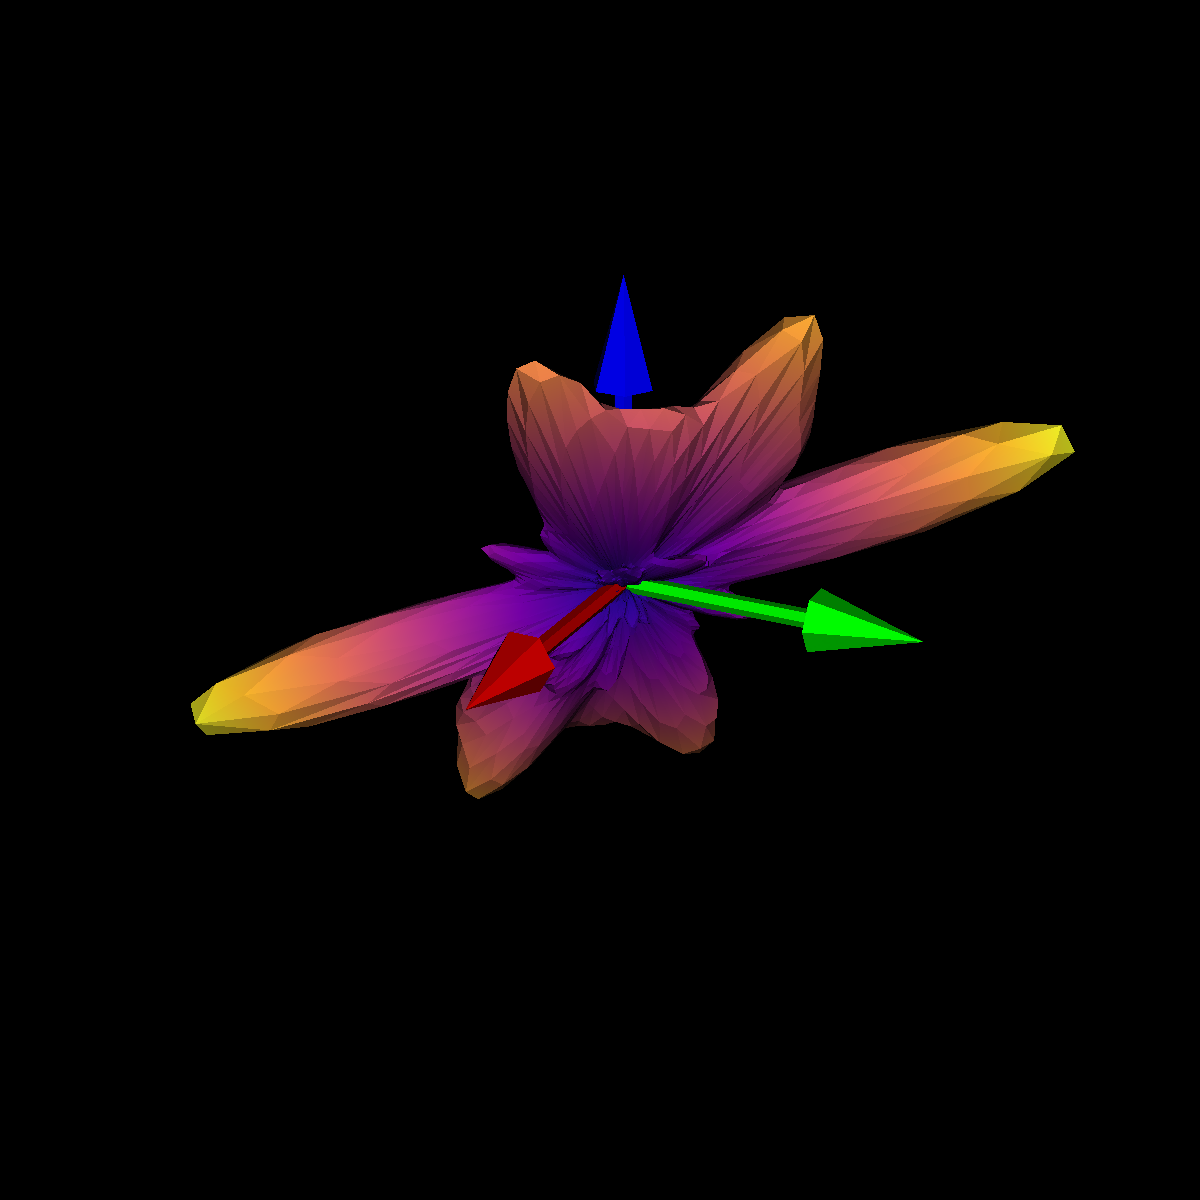
\includegraphics[width=0.9\linewidth]{../odf_comparison/delta_odf_sh}
    \caption{Delta}
    \label{fig:delta}
  \end{subfigure}
  \hspace{0.5em}
  \begin{subfigure}[b]{0.48\textwidth}
    \centering
    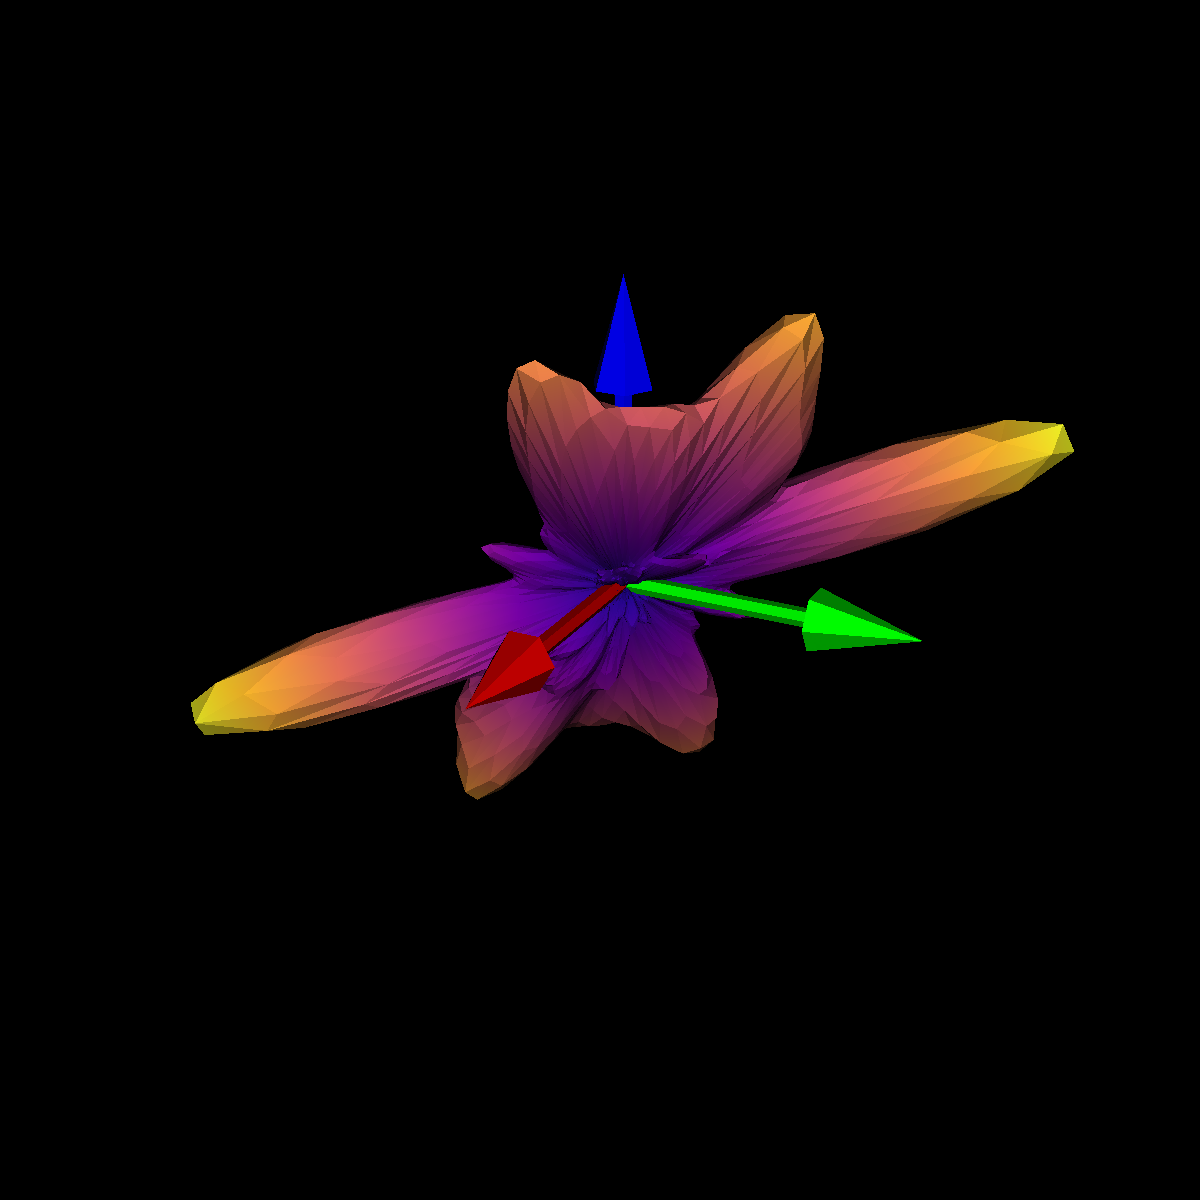
\includegraphics[width=0.9\linewidth]{../odf_comparison/hist_odf_sh}
    \caption{Binned}
    \label{fig:binned}
  \end{subfigure}
  \caption{SH FOD representations}
  \label{fig:vis_comparison}
\end{figure}

Figure~\ref{fig:vis_comparison} shows a comparison of the SH representation of
the FODs calculated with the delta function method (Fig~\ref{fig:delta},
Eqn~\ref{eq:1}) and the spherical binning method (Fig~\ref{fig:binned},
Eqn~\ref{eq:3}). The binned FOD was calculated using $N=6500$ sample points, and
both FODs were also plotted on a sphere with the same $N=6500$ points. Bth SH
representations look like spherically ``blurred'' versions of
Figure~\ref{fig:fod_even}, as we expect.

Visually, the difference between the two FODs are negligible. This difference is
quantified in Figure~\ref{fig:rmse} as the root mean squared error (RMSE) of the
SH coefficients, plotted as a function of the number of sampling points. The RMSE is
calculated as
\begin{align}
  \label{eq:rmse}
  \text{RMSE} = \sqrt{\frac{1}{N_{SH}}\sum_{l,m} \left[c_{lm}^{\delta} - c_{lm}^{b}(N)\right]^2},
\end{align}
where $N_{SH}=231$ is the total number of SH coefficients,
$c_{lm}^{\delta}$ is the SH coefficient for $l$ and $m$ calculated with the delta
function method and $c_{lm}^b(N)$ is the SH coefficient for $l$ and $m$ calculated
with the binned method using $N$ sample points.

\begin{figure}[h]
  \centering
  \begin{subfigure}[b]{0.48\textwidth}
    \centering
    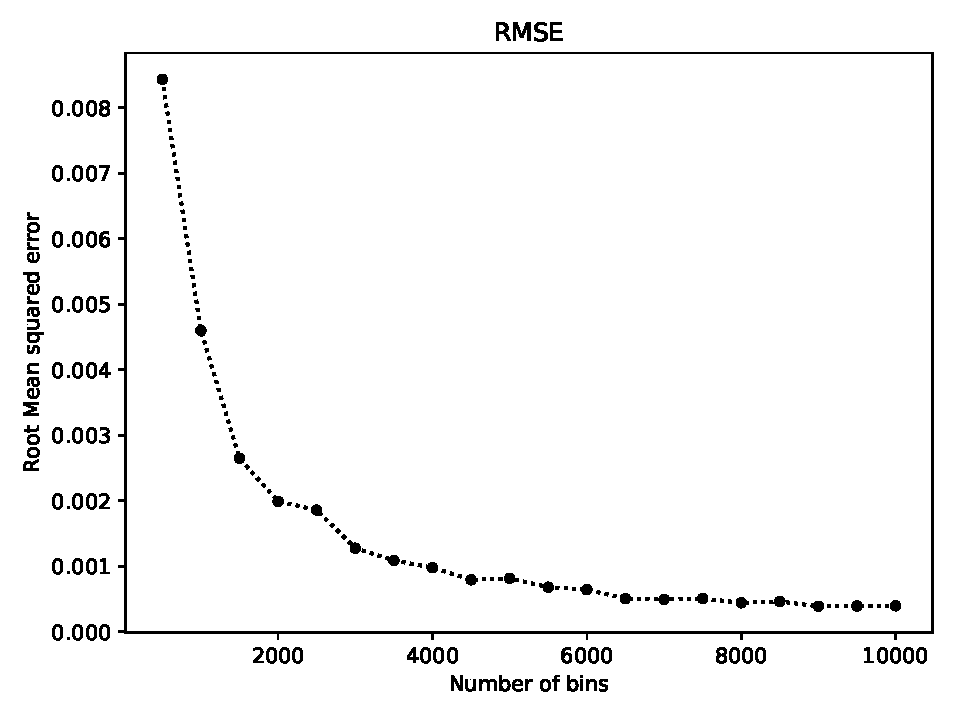
\includegraphics[width=0.9\linewidth]{../plot_rmse/rmse}
    \caption{RMSE}
    \label{fig:rmse}
  \end{subfigure}
  \hspace{0.5em}
  \begin{subfigure}[b]{0.48\textwidth}
    \centering
    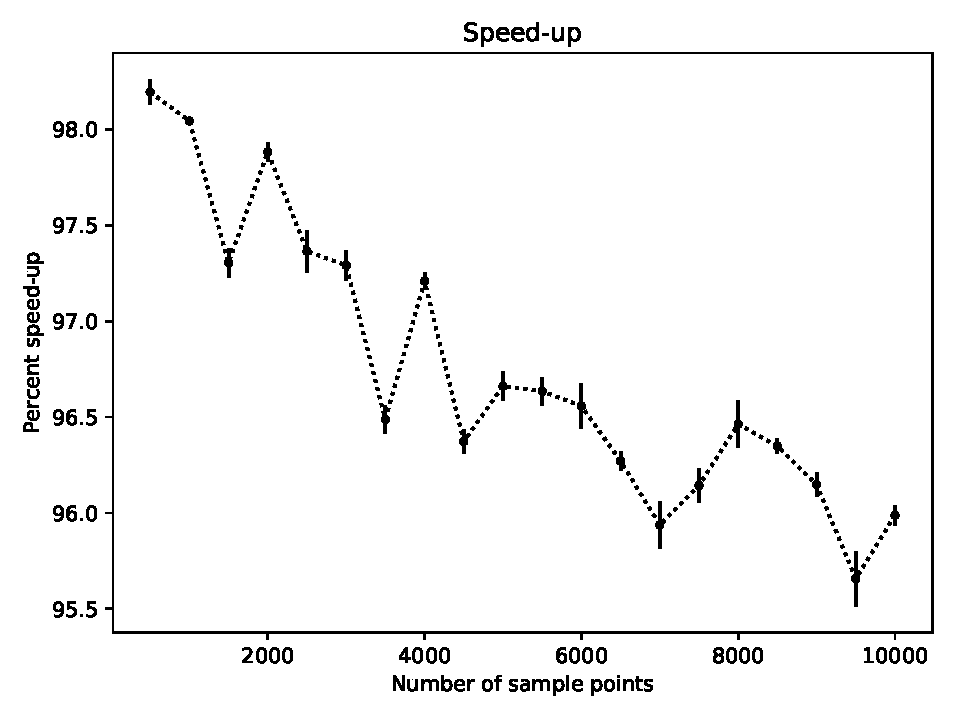
\includegraphics[width=0.9\linewidth]{../plot_speedup/speedup}
    \caption{Speedup}
    \label{fig:speedup}
  \end{subfigure}
  \caption{Performance metrics}
  \label{fig:metrics}
\end{figure}
Figure~\ref{fig:speedup} shows the corresponding speed-up of computation time
between the two methods. For each $N$, a single ``best-case'' time measurement
was recorded as the lowest time of three separate executions. The average time
$\bar{t}_N$ and error $\sigma_N$ were taken as the mean and standard deviation
of ten of these lowest times; thus, the coefficients were calculated a total of
30 times for each $N$, as well as for the delta method. The percent speed-up (SU$_N$)
was then calculated as
\begin{align}
  \text{SU}_N = \left(1 - \frac{\bar{t}_N}{\bar{t}_{\delta}}\right)\times 100,
\end{align}
where $\bar{t}_{\delta}$ is the mean execution time for the delta method. The error
in SU$_N$ was calculated by adding the relative errors of the binned and delta times:
\begin{align}
  \sigma_{SU,N} = \left(\frac{\sigma_N}{\bar{t}_N} + \frac{\sigma_{\delta}}{\bar{t}_{\delta}}\right)\times \text{SU}_N
\end{align}

\section{Conclusion}
Together, these plots show that for an adequate number of sampling points, the
binned FOD method approaches a 100\% speedup with very little loss in accuracy.
The percent speedup generally decreases with increasing $N$, as expected, though
it stays consistently over 95\%. The RMSE seems to level off after around
$N=6500$. With this level of accuracy, the FODs could be calculated across the
whole brain in a much more managable computation time of \textapprox 140 hours.
Spread across multiple nodes, this could be completed in less than a day. 


\bibliographystyle{ieeetr}
\bibliography{SH_speedup_notes}  
\end{document}